\documentclass{beamer}
% to typeset the presentation as a handout uncomment:
%\documentclass{article}
%\usepackage{beamerarticle}

\usepackage{graphicx,hyperref,url}
\usepackage{color,colortbl}
\usepackage{hyperref}

\newcommand{\myhref}[2]{{\color{blue}\href{#1}{#2}}} 

\usecolortheme{beaver}
\usetheme{Goettingen}
\setbeamercolor{navigation symbols}{fg=red, bg=black}

\usefonttheme[onlymath]{serif}

\makeatletter
\setbeamertemplate{sidebar canvas \beamer@sidebarside}%
                  [vertical shading][top=red,bottom=gray]
\makeatother

\title{Monitoring the urban noise environment}
\subtitle{joint with the IoT Lab, Civic Innovation YYC}

\author{D. Richert, H. Leung}
\institute[University of Calgary]
{
  Department of Electrical and Computer Engineering\\
  Schulich School of Engineering\\University of Calgary
}

\logo{%
    
\includegraphics[width=2cm,height=2cm,keepaspectratio]{figures/uc_logo} \hspace*{1cm} {\color{black} August 24, 2017} \hspace*{1cm} 
\includegraphics[width=2cm,height=2cm,keepaspectratio]{figures/schulich}
}

\date{\scalebox{1}{\insertlogo}}

\AtBeginSection[]
{
  \begin{frame}<beamer>{Outline}
    \tableofcontents[currentsection,currentsubsection]
  \end{frame}
}

\begin{document}

\begin{frame}
  \titlepage
\end{frame}

\begin{frame}{Outline}
  \tableofcontents
\end{frame}

\section{Project Motivation}

    \begin{frame}{Project Motivation - LPWAN Project}
        \begin{itemize}
            \item Establish the City of Calgary as a leader in the smart city movement
            \item Assess how LPWAN technology can be used to improve the quality of life for citizens of Calgary
            \item Test the capabilities of LPWAN to determine which smart city applications the technology is best-suited for
            \item Speed up concept-to-development and minimize costly mistakes of adopting the wrong IoT solution
            \item Implement and validate futuristic algorithms on a real sensor network
            \item Strengthen the  relationship between Civic Innovation YYC and the U of C 
        \end{itemize}
    \end{frame}

    \begin{frame}{Project Motivation - acoustic monitoring}
        \begin{itemize}
            \item Unwanted noise in urban environments has negative health effects
            \begin{itemize}
                \item loss of sleep, disruption to relaxation and social gatherings, hearing loss, high blood pressure, and more
            \end{itemize}
            \item City noise codes aim to reduce noise pollution, but violations of the code are difficult to catch
            \item Continuous monitoring of noise is rare. Noise assessments are complaint driven.
            \item Noise data also contains information about the happenings within a city.
                \begin{itemize}
                    \item traffic noise, construction noise, persons in distress, car accidents, etc.
                \end{itemize}
            \item Acoustic monitoring promises to be a good application for environmental monitoring using LPWAN.
        \end{itemize}
    \end{frame}

\section{Relevant case studies}
    
    \subsection{SONYC}
        
    \begin{frame}{Sounds of New York City (SONYC) - project objectives}
        From the project \myhref{https://wp.nyu.edu/sonyc}{website}...
        \vfill 
        Objectives: to create technological solutions for
        \begin{itemize}
            \item the systematic, constant monitoring of noise pollution at the city scale
            \item the accurate description of acoustic environments in terms of its composing sources
            \item broadening citizen participation in noise reporting and mitigation
            \item enabling city agencies to take effective, information-driven action for noise mitigation.
        \end{itemize}
    \end{frame}  
    
    \begin{frame}{Sounds of New York City (SONYC) - project overview}
        \begin{center}
            \begin{figure}
                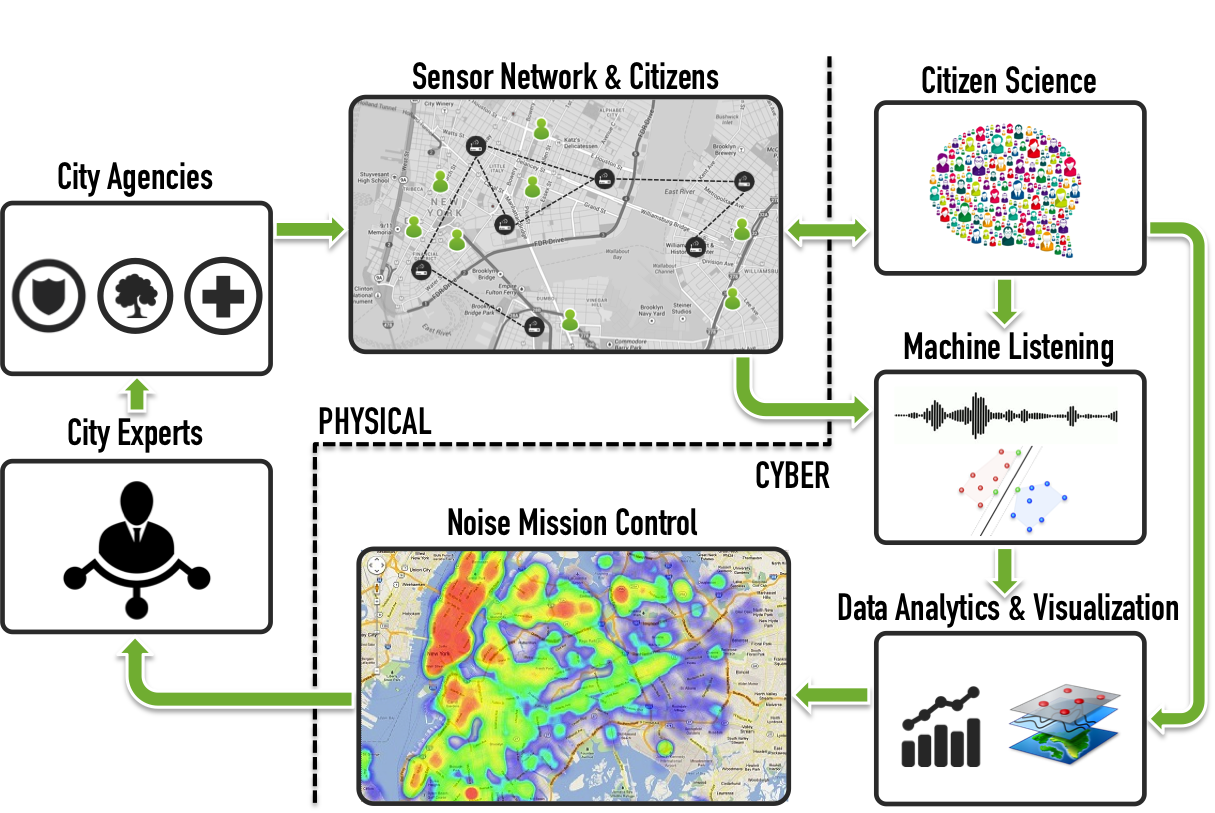
\includegraphics[scale=0.4]{figures/sonyc.png}
                \caption{SONYC project overview (image taken from the project \myhref{https://wp.nyu.edu/sonyc}{website})}
            \end{figure}
        \end{center}
    \end{frame}
    
    \begin{frame}{Sounds of New York City (SONYC) - prototype}
        \begin{center} 
            \begin{figure}
                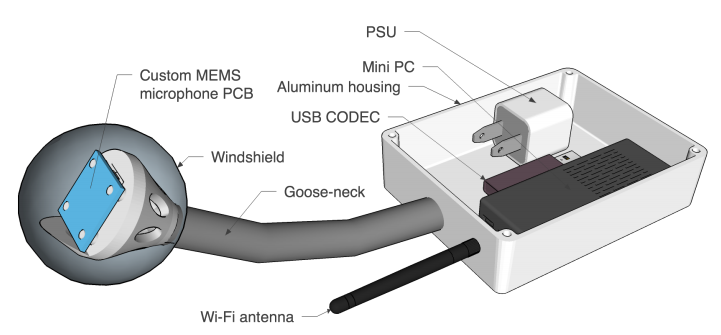
\includegraphics[scale=0.5]{figures/sonyc_prototype}
                \caption{SONYC sensor unit prototype (image taken from the project \myhref{https://wp.nyu.edu/sonyc}{website})}
            \end{figure}
        \end{center}
    \end{frame}
    
    \begin{frame}{Sounds of New York City - project impact \& results}
        \begin{itemize}
            \item granted a \$4.6 million Fontier award from the NSF to advance research in cyber-physical systems for smart cities
            \item NYC BigApps finalist - a civic innovation competition in NYC to improve the city.
            \item supports 15 academics
            \item partners with NYC Environmental Protection, NYC Health, and Downtown Alliance.
        \end{itemize}
    \end{frame}
        
    \subsection{RUMEUR network}

    \begin{frame}{RUMEUR network - project objectives} 
        Designed and maintained by Bruitparif, a non-profit based in Paris. Project objectives (from the project's \myhref{http://www.conforg.fr/euronoise2015/proceedings/data/articles/000043.pdf}{EuroNoise conference paper})  
        \begin{itemize}
            \item Better understand noise phenomena: factors that influence noise, changes over time, exposure data correlated to socio-economic impacts
            \item Evaluate noise mitigation measures: obtain indicators for tracking the impact of mitigation policies, anticipate impact of future projects.
            \item Disseminate noise information to the public
        \end{itemize}
     \end{frame} 
     
    \begin{frame}{RUMEUR network - project overview} 
        \begin{minipage}{0.5\linewidth}
        \begin{itemize}
            \item 45 long-term high precision monitoring terminals and 350 short-term terminals
            \item Focus is on traffic and aircraft noise
            \item Data transmission over cellular network
            \item Real-time data dissemination through their \myhref{http://rumeur.bruitparif.fr/}{web application}  
        \end{itemize} 
        \end{minipage}
        \begin{minipage}{0.45\linewidth}
            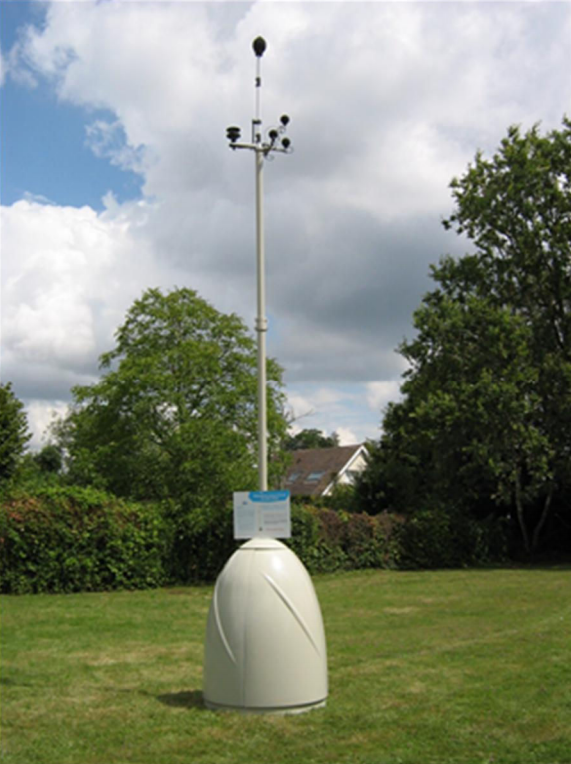
\includegraphics[scale=0.3]{figures/rumeur_longterm}
        \end{minipage}
    \end{frame}
    
    \begin{frame}{RUMEUR network - data dissemination}         
        \begin{center}
            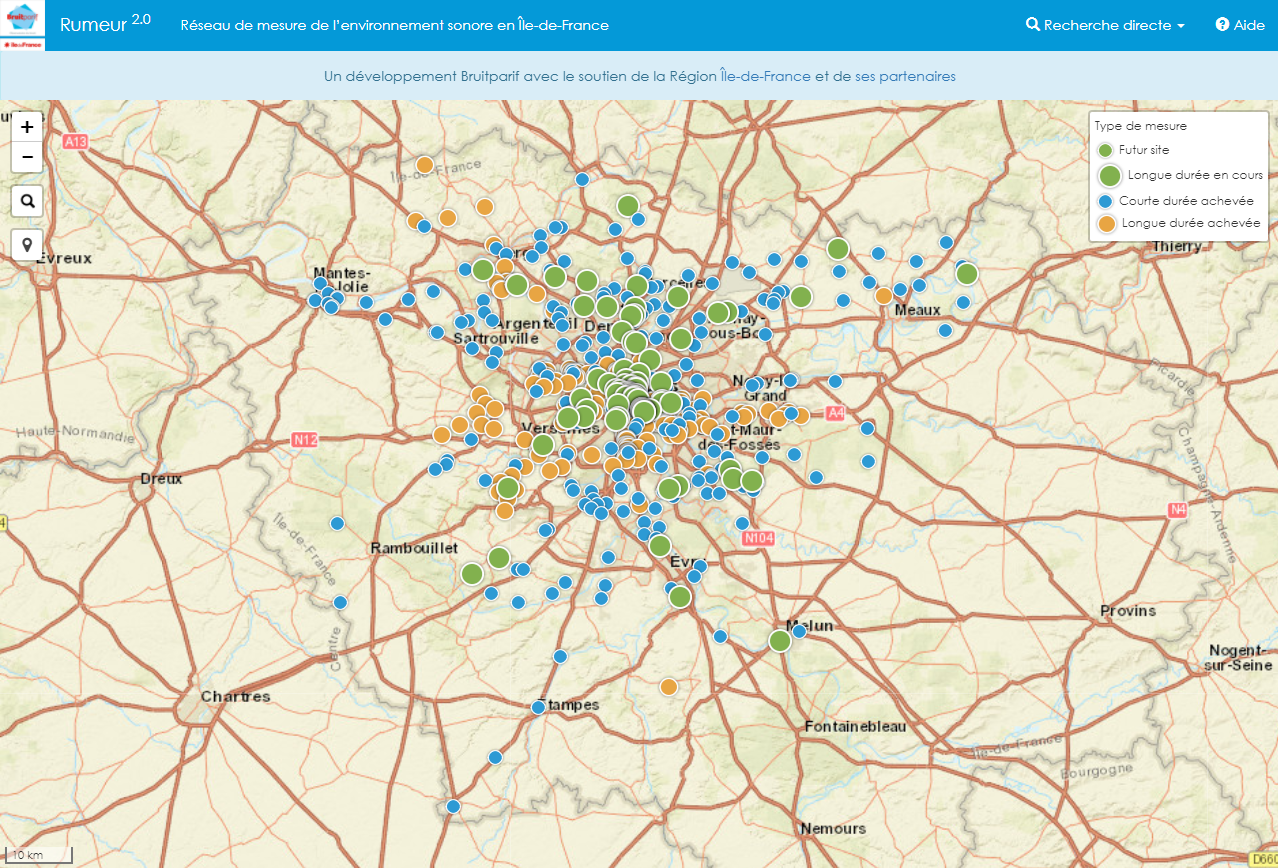
\includegraphics[scale=0.28]{figures/rumeur2}
        \end{center}
    \end{frame}
    
    \begin{frame}{RUMEUR network - data dissemination}         
        \begin{center}
            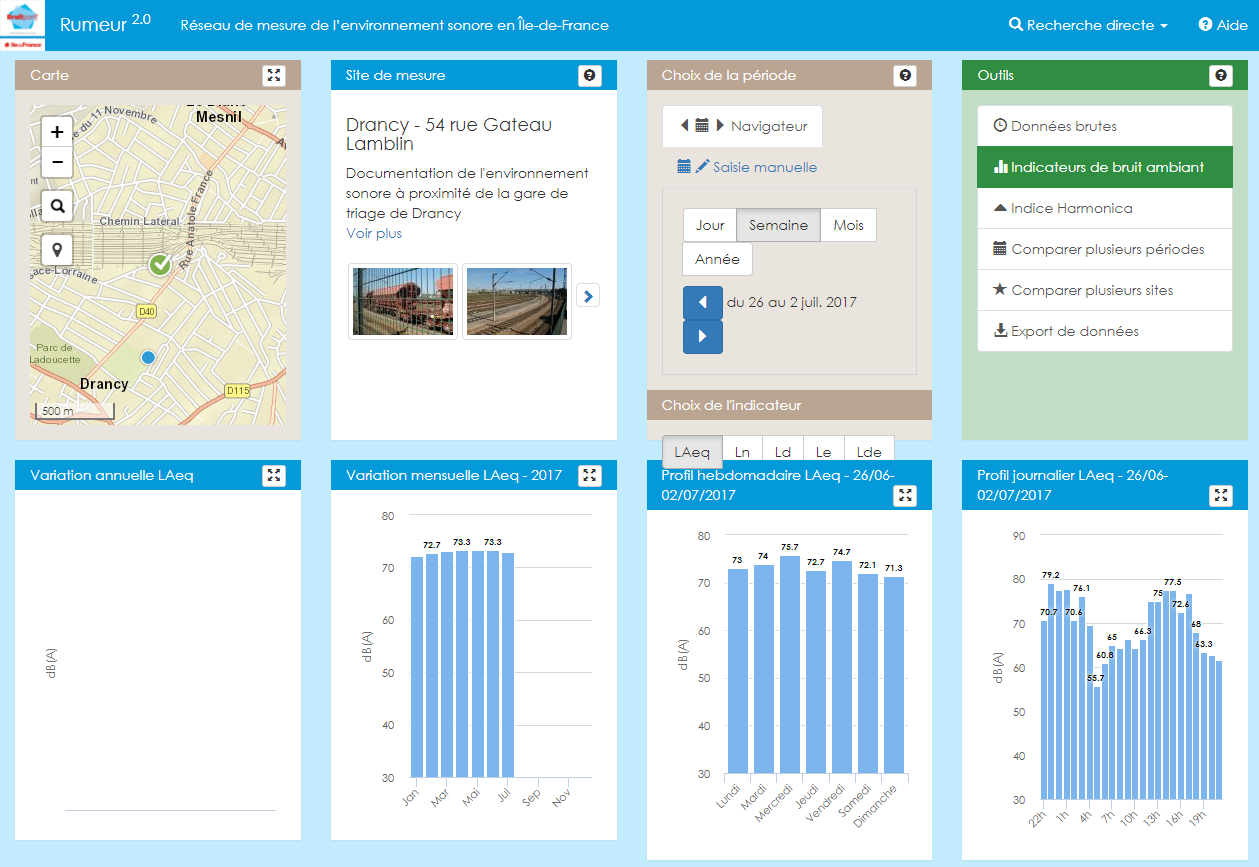
\includegraphics[scale=0.28]{figures/rumeur1}
        \end{center}
    \end{frame}
    
    \begin{frame}{RUMEUR network - project impact \& results}
        \begin{itemize}
            \item recipient of the Best Life Environment Project  
            \item recipient of the Decibel D'Or award by the National Council of Noise
        \end{itemize}
    \end{frame}

\section{Acoustic sensing basics}

    \begin{frame}{Acoustic sensing basics}
        \begin{itemize}
            \item Frequency range of human hearing is 20Hz-20kHz, but most sensitive in the 2-5kHz range
            \item Sound level range of human hearing 0dB - 85dB (above 85dB is dangerous)
            \item What is a dB? A logarithmic ratio of two values. In acoustics, the equivalent sound pressure level is used:
            \begin{align*}
                L_{eq} = 20 \log_{10} \bigg( \frac{1}{t_2-t_1}\int_{t_1}^{t_2} \frac{p_1}{p_0} dt \bigg)
            \end{align*}  
            where $p_1$ is the rms sound pressure and $p_0$ is a reference sound pressure ($20 \mu Pa$). 
        \end{itemize}
    \end{frame}

    \begin{frame}{Acoustic sensing basics}
        \begin{itemize}
            \item For environmental monitoring, a weighted sound level is used (dBA, e.g.)
            \item The (lower) threshold of human hearing is frequency dependant - at the same sound pressures, lower \& higher frequencies seem quieter to a human
            \item Weighting lower \& higher frequencies less give a more representative sound level:
            \begin{center}
            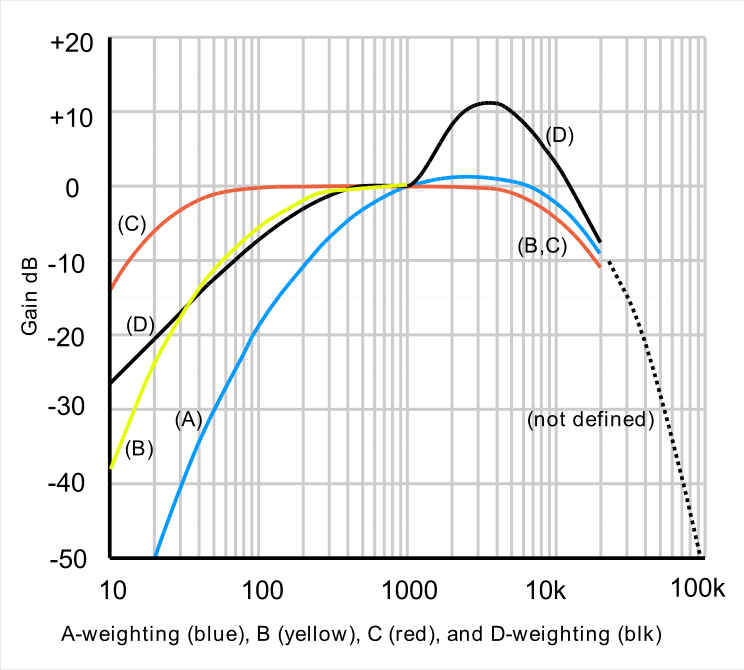
\includegraphics[scale=0.175]{figures/acoustic_weighting_curves.png}
            \end{center}
            
        \end{itemize}
    \end{frame}
    
    \begin{frame}{Acoustic sensing basics - sound level meter standards}
        IEC 61672-1 is the sound level meter (SLM) standard for sensors used for legally enforceable acoustic monitoring purposes. Includes specifications for device:
        \begin{itemize}
            \item frequency response tolerance limits
            \item self generated noise
            \item linearity 
            \item type 1 devices (precision) vs. type 2 devices (general purpose)
            \item industry standard tests that can be used to evaluate sensor performance
        \end{itemize}
    \end{frame}
    
    \begin{frame}{Acoustic sensing basics - sound level meter standards}
        \begin{itemize}
            \item {\bf Class 1 - precision measurements}: accurate, reliable, enforceable acoustic monitoring. Sensors alone cost \$1,000-2,000. Required accuracy of $\pm$1dBA at 1kHz. Pre-amplifiers and high voltages required for operation.
            \item {\bf Class 2 - general purpose measurements}: minimum requirement for OSHA noise measurements and general purpose noise surveys. Required accuracy of $\pm$2dBA at 1kHz.
            \item {\bf Class 3 - low-cost}: Sensors can be very cheap (as low as \$1). Measure noise levels in the 40-100dBA range with $\pm$3dBA accuracy or worse. Enables scalablity.
        \end{itemize}
    \end{frame}

    \begin{frame}{Acoustic sensing basics - City of Calgary Bylaws}
        \begin{itemize}
            \item City of Calgary Bylaw - continuous sound in downtown, for example: 
           \begin{center} \fbox{\begin{minipage}{0.75\linewidth}
                \emph{No person shall cause continuous sound that exceeds 75dBA during the day-time (60dBA during the night-time)}
            \end{minipage}}
            \end{center}
            \begin{itemize}
                \item Continuous sound = continuous duration over a 3 minute period, or sporadically for a total of 3 minutes over a 15 minute period. 
                \item Sound level must exceed 5dBA over ambient before it becomes an offence
            \end{itemize}
            \item For enforcement purposes, a type 2 sound level meter must be used 
        \end{itemize}
    \end{frame}

\section{LPWAN basics}

    \begin{frame}{LPWAN - a type of wireless telecommunication}
        \begin{itemize}
            \item Low data throughput. Mostly uplink traffic with small 10-200B packets 
            \item Low power (several years of operation with a single battery charge is theoretically possible)
            \item Long range ($\approx$ 5km in urban areas, $\approx$ 15km in open areas)
            \item LoRa is a specific LPWAN technology (SIGFOX is another, for example)
        \end{itemize}
    \end{frame}

    \begin{frame}{LoRa - proprietary physical layer}
        Semtech \alert{Lo}ng \alert{Ra}nge physical layer
        \begin{itemize}
            \item Sub-GHz (unlicensed ISM radio bands, 902-928MHz in Canada) bi-directional point-to-point wireless link
            \begin{itemize}
                \item The band is divided into 8 sub-bands that each have 8x125 kHz uplink channels, 1x500 kHz uplink channel and 1x500 kHz downlink channel.
            \end{itemize}
            \item 13.5mA RX current, 124mA TX current
        \end{itemize}
    \end{frame}
    
    \begin{frame}{LoRaWAN - medium access control}
        \begin{itemize}
            \item Devices are asynchronous and transmit when they have data available to send (ALOHA protocol). 
            \item Data transmitted by an end-node device is received by multiple gateways, which forward the data packets to a centralized network server. 
            \item The network server filters duplicate packets, performs security checks, and manages the network. 
        \end{itemize}
    \end{frame}
    
\section{Project deliverables \& timeline}

    \begin{frame}{Agreed upon deliverables}
        From the project proposal:
        \begin{itemize} 
            \item Design and construction of 15 acoustic sensing units
            \item Deployment of sensing units
            \item Real-time reporting of data to LoRaWAN gateway
            \item Data storage on cloud database
            \item Model for characterization of acoustic sources (used for in-situ processing)
            \item Data visualization and automated dashboard tool for real-time mapping of data
            \item Spatial and temporal model of acoustic emissions within study area
            \item Report on the project outcomes and future directions
        \end{itemize}
    \end{frame}

    % \begin{frame}{Project timeline: Aug. 1 - Dec. 31}
    %     \hspace*{-0.4cm}\tiny{\begin{tabular}{r|p{0.1cm}p{0.1cm}p{0.1cm}p{0.1cm}p{0.1cm}p{0.1cm}p{0.1cm}p{0.1cm}p{0.1cm}p{0.1cm}p{0.1cm}|}
    %              \multicolumn{2}{r}{Week \#} & \multicolumn{10}{c}{} 
    %             \\ Task & 1 & 2 & 3 & 4 & 5 & 6 & 7 & 8 & 9 & 10 & 11 \\ \hline 
    %             Sensor unit specs & \cellcolor{lime} & & & & & & & & & & \\ \cline{1-1}
    %             In-situ processing spec & \cellcolor{lime} & \cellcolor{cyan} & & & & & & & & & \\ \cline{1-1} 
    %             Design units & & \cellcolor{cyan} & \cellcolor{cyan} & \cellcolor{cyan} & \cellcolor{cyan} & & & & & & \\  \cline{1-1} 
    %             Design in-situ processing & & \cellcolor{cyan} & \cellcolor{cyan} & \cellcolor{cyan} & \cellcolor{cyan} &  &  & \cellcolor{cyan} & \cellcolor{cyan} & & \\ \cline{1-1}  
    %             Test prototype & & & & & & \cellcolor{cyan} & \cellcolor{cyan} & \cellcolor{cyan} & \cellcolor{cyan} & & \\ \cline{1-1} 
    %             Order all units & & & & & & & & & & \cellcolor{cyan} & \cellcolor{cyan}  \\
    %             \cline{1-1} Data storage system & & & & & & & & & & \cellcolor{cyan}& \cellcolor{cyan} \\ \cline{1-1}
    %             Classification models & & & & & & & & & & & \cellcolor{cyan} \\   \cline{1-1} 
    %             Units deployed & & & & & & & & & & & \\ \cline{1-1}
    %             Data visualization tool & & & & & & & & & & & \\ \cline{1-1}
    %             Process data & & & & & & & & & & & \\ \cline{1-1}
    %             Spatial/temporal map & & & & & & & & & & & \\ \cline{1-1}
    %             Report & & & & & & & & & & & \\ \hline
    %         \end{tabular}} \medskip \\  
    %         \hspace*{1.7cm}\tiny{\begin{tabular}{r|p{0.1cm}p{0.1cm}p{0.1cm}p{0.1cm}p{0.1cm}p{0.1cm}p{0.1cm}p{0.1cm}p{0.1cm}p{0.1cm}p{0.1cm}|}
    %              \multicolumn{2}{r}{Week \#} & \multicolumn{10}{c}{} 
    %             \\ Task & 12 & 13 & 14 & 15 & 16 & 17 & 18 & 19 & 20 & 21 & 22 \\ \hline 
    %             Sensor unit specs & & & & & & & & & & & \\ \cline{1-1}
    %             In-situ processing spec & & & & & & & & & & & \\ \cline{1-1} 
    %             Design units & & & & & & & & & & & \\  \cline{1-1} 
    %             Design in-situ processing & & & & & & & & & & & \\ \cline{1-1}  
    %             Test prototype & & & & & & & & & & & \\
    %             \cline{1-1} 
    %             Order all units & & & & & & & & & & & \\ \cline{1-1} Data storage system & & & & & & & & & & & \\ \cline{1-1}
    %             Classification models & \cellcolor{cyan} & \cellcolor{cyan} & \cellcolor{cyan} & & & & & & & &  \\  \cline{1-1} 
    %             Units deployed & \cellcolor{cyan} & \cellcolor{cyan} & \cellcolor{cyan} & \cellcolor{cyan} & \cellcolor{cyan} & \cellcolor{cyan} & \cellcolor{cyan}  & \cellcolor{cyan} & \cellcolor{cyan} & & \\ \cline{1-1}
    %             Data visualization tool & & & \cellcolor{cyan} & \cellcolor{cyan} & \cellcolor{cyan} & & & & & & \\ \cline{1-1}
    %             Process data & & & & \cellcolor{cyan} & \cellcolor{cyan} & \cellcolor{cyan} & \cellcolor{cyan} & \cellcolor{cyan} & \cellcolor{cyan} & \cellcolor{cyan} & \\ \cline{1-1}
    %             Spatial/temporal map & & & & & & & & \cellcolor{cyan} & \cellcolor{cyan} & \cellcolor{cyan} & \\ \cline{1-1}
    %             Report & & & & & & & & & & \cellcolor{cyan} & \cellcolor{cyan}\\ \hline
    %         \end{tabular}}
    % \end{frame}
    
    \begin{frame}{Project timeline: Aug. 28 - Jan. 31}
        \begin{center}
        \scriptsize{\begin{tabular}{l|p{0.1cm}p{0.1cm}p{0.1cm}p{0.1cm}p{0.1cm}p{0.1cm}p{0.1cm}p{0.1cm}p{0.1cm}p{0.1cm}p{0.1cm}|}
                 \multicolumn{2}{r}{Week \#} & \multicolumn{10}{c}{} 
                \\ Phase & 1 & 3 & 5 & 7 & 9 & 11 & 13 & 15 & 17 & 19 & 21 \\ \hline 
                1: Sensor unit design specs & \cellcolor{cyan} & \cellcolor{cyan} & \cellcolor{cyan} & \cellcolor{cyan} & \cellcolor{cyan} & \cellcolor{cyan} & & & & & \\ \cline{1-1}
                2: Data management system &  & & \cellcolor{cyan} & \cellcolor{cyan} & \cellcolor{cyan} & \cellcolor{cyan} & \cellcolor{cyan} & \cellcolor{cyan} & & & \\ \cline{1-1} 
                3: Assembly and deployment & &  &  &  &  & &  & \cellcolor{cyan} & \cellcolor{cyan} & \cellcolor{cyan} & \cellcolor{cyan} \\  \cline{1-1} 
                4: Data analysis and reporting & & & &  & & & & & & \cellcolor{cyan} & \cellcolor{cyan}  \\ \hline
            \end{tabular}} 
            \end{center}
    \end{frame}

\section{Sensor unit functional specs}

    \begin{frame}{Functional specifications - hardware}
    The sensor unit shall ... 
        \begin{itemize}
            \item measure sound pressure levels with a comparable level of accuracy to City of Calgary Bylaw standards 
            \item transmit processed audio data and metadata to a City of Calgary LoRaWAN radio gateway
            \item receive acknowledgment and control signals from a City of Calgary LoRaWAN radio gateway
            \item maintain its full functionality for at least 8 weeks without human intervention
            \item operate year round in typical Calgary weather (electronics and battery should operate down to -20$^\circ$C). 
            \item cost less than \$200 per sensor node
            \item not require a wired connection to any utility
            \item be capable of being deployed within 30 minutes of arriving at a proposed location
        \end{itemize}
    \end{frame}
    
    \begin{frame}{Functional specifications - algorithms}
    The sensor unit shall ... 
        \begin{itemize}
            \item randomly sample 30 seconds (?) of acoustic data 
            \item increase the sampling frequency autonomously when changes are detected in the acoustic environment
            \item perform in-situ signal processing on audio measurements, including:
                \begin{itemize}
                    \item filtering
                    \item spectral decomposition
                    \item A-weighting
                    \item noise source characterization
                \end{itemize} 
            \item transmit data to the LoRaWAN gateway when changes in the acoustic environment are detected
            \item autonomously update sensor unit parameters based on control signals received from the LoRaWAN gateway
        \end{itemize}
    \end{frame}

\section{Proposed hardware}

    \begin{frame}{Proposed hardware - off-the-shelf options}
        There are no off-the-shelf solutions that will satisfy the functional specifications. The best candidates include: \\
        \vspace*{0.25cm}
        \begin{minipage}{0.48\linewidth}
        \begin{itemize}
            \item \myhref{http://www.libelium.com/development/waspmote}{Waspmote by Libelium}: $\approx$ \$300, minimum operating temperature is $-10^{\circ}$C, limited ability to add custom functionality. 
        \end{itemize}
        \end{minipage}
        \begin{minipage}{0.48\linewidth}
            \begin{center}
                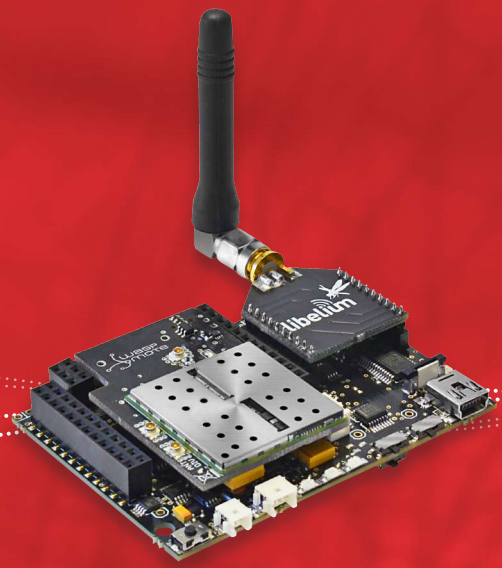
\includegraphics[scale=0.2]{figures/wasp.PNG}
            \end{center}
        \end{minipage} \\ \vspace*{0.5cm} \hline \vspace*{0.5cm}
        \begin{minipage}{0.48\linewidth}
            \begin{center}
                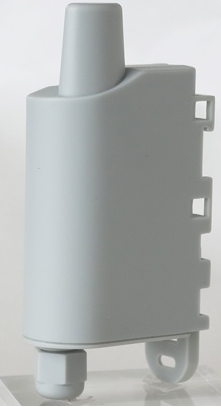
\includegraphics[scale=0.2]{figures/adeunis.PNG}
            \end{center}
        \end{minipage}
        \begin{minipage}{0.48\linewidth}
        \begin{itemize}
            \item \myhref{http://www.adeunis-rf.com/en/products/lorawan-products}{Adeunis RF LoRaWAN transceiver}: barebones and rugged design, in-situ processing not possible.
        \end{itemize}
        \end{minipage}
    \end{frame}

    \begin{frame}{Proposed hardware - prototype}
        LoRa Tx/Rx: \myhref{http://www.microchip.com/DevelopmentTools/ProductDetails.aspx?PartNO=RN-2903-PICTAIL}{Microchip RN2903 LoRa Technology PICtail}
        \vfill
        \begin{center}
            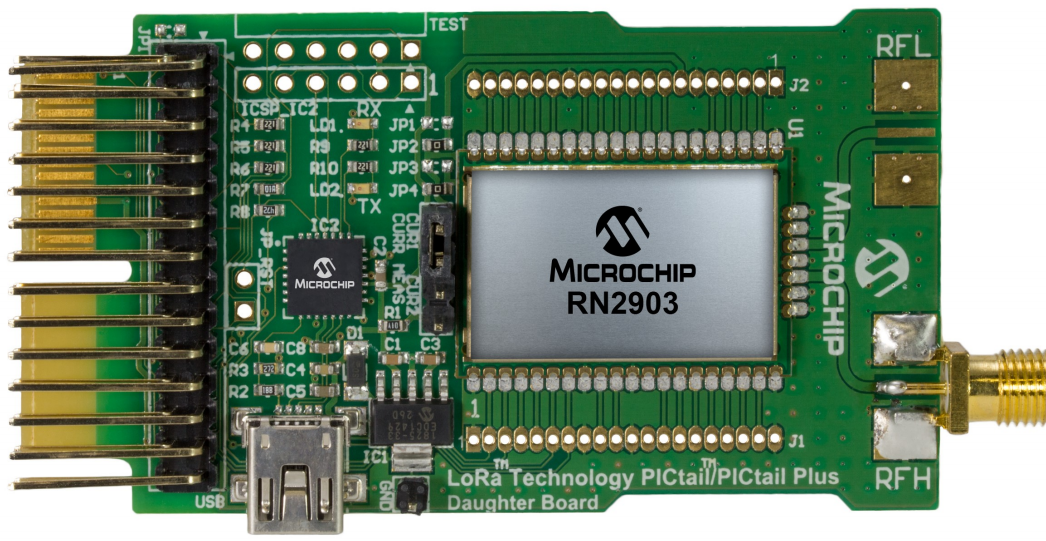
\includegraphics[scale=0.2]{figures/microchip.PNG}
        \end{center}
        \vfill 
        \begin{itemize}
            \item Features Microchip's RN2903 LoRa 915MHz transceiver module
            \item PICtail connection interface
            \item On-board PIC18 MCU
            \item supply current measurement points
            \item \$82
        \end{itemize}
    \end{frame}
    
    \begin{frame}{Proposed hardware - prototype}
        
        Development kit: \myhref{http://www.microchip.com/DevelopmentTools/ProductDetails.aspx?PartNO=DM240001-3}{Microchip Explorer 16/32}
        \vspace*{-0.7cm}
        \begin{center}
            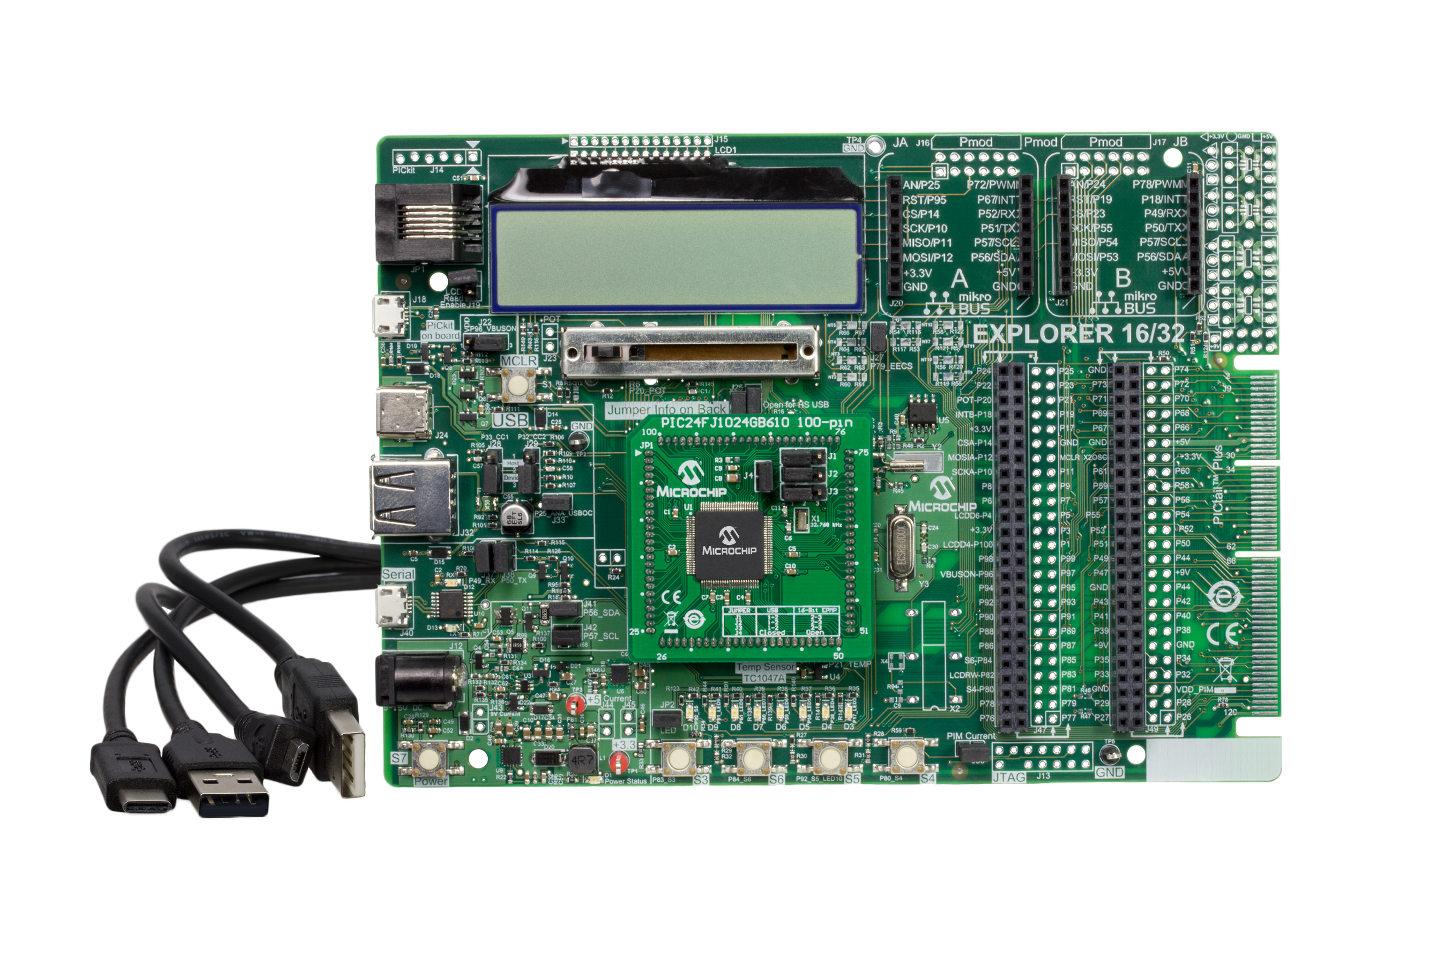
\includegraphics[scale=0.2]{figures/microchiptechnologyinc_35116794972.png}
        \end{center}
        \vspace*{-1cm}
        \begin{itemize}
            \item Supports processor plug-in modules
            \item PICtail connection interface
            \item LCD display
            \item supply current measurement points
            \item \$138 (Dev. kit) + \$32 (\myhref{http://www.microchip.com/DevelopmentTools/ProductDetails.aspx?PartNO=MA240023}{processor}) + \$68 (\myhref{https://www.digikey.ca/product-detail/en/microchip-technology/PG164130/PG164130-ND/2171224}{programmer})
        \end{itemize}
    \end{frame}

    \begin{frame}{Proposed hardware - prototype}
        Microphone sensor: \myhref{https://www.invensense.com/products/analog/ics-40720/}{InvenSense ICS-40720 Evaluation Board}
        \begin{center}
            \begin{minipage}{0.45\linewidth}
            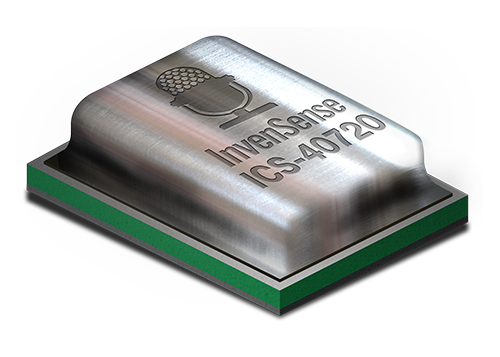
\includegraphics[scale=0.2]{figures/rp-ics-40720.png} 
            \end{minipage}
            \begin{minipage}{0.45\linewidth}
            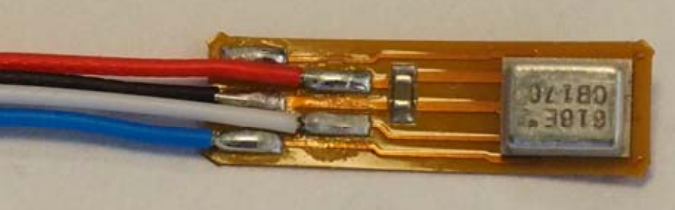
\includegraphics[scale=0.2]{figures/invensense_eval.PNG}
            \end{minipage}
        \end{center}
        \begin{itemize}
            \item accuracy of $\pm$2dB
            \item frequency response from 75Hz-20kHz
            \item 285$\mu$A supply current, 1.5-3.6V supply voltage
            \item high SNR of 70dBA
            \item dynamic range of 124dB
            \item sensitivity of -32dBV
            \item \$44
        \end{itemize}
    \end{frame}
    
    \begin{frame}{Proposed hardware - final design}
    \smallskip \\ 
        {\footnotesize{\begin{center}
        \begin{tabular}{|l|l|} \hline 
            {\bf Part (with URL)} & {\bf Price} \\ \hline 
            LoRa Tx/Rx (\myhref{http://www.microchip.com/wwwproducts/en/RN2903}{Microchip RN2903}) & \$14.57 \\ 
            \hline Microphone (\myhref{https://www.invensense.com/products/analog/ics-40720/}{InvenSense ICS-40720}) & \$5.00 \\ \hline 
            Microcontroller (\myhref{http://www.microchip.com/wwwproducts/en/PIC24FJ1024GB610}{Microchip PIC24FJ1024GB610}) & \$5.41 \\ \hline
            Protective case (\myhref{https://www.digikey.ca/product-detail/en/hammond-manufacturing/1550WE/HM1214-ND/2211564}{Hammond Manufacturing 1550WE}) & \$18.70 \\ \hline 
            Antenna (\myhref{https://www.digikey.ca/product-detail/en/microchip-technology/RN-SMA4-RP/740-1033-ND/2207396}{Microchip RN-SMA4-RP}) & \$7.65 \\ \hline Microphone mount \& windshield & \$5.00 \\ \hline
            Lithium-thionyl chloride battery (\myhref{http://www.tadiranbatteries.de/pdf/lithium-thionyl-chloride-batteries/SL-2790.pdf}{Tadiran SL-2790}) & \$42.00 \\ \hline Miscellaneous (parts \& assembly) & \$20.00 \\ \hline  
            Total: & \$118.33 \\ \hline 
        \end{tabular}
        \end{center}}}
    \end{frame}
    
\section{Questions/feedback}

    \begin{frame}{Questions/feedback}
        \begin{center}
            
\includegraphics[scale=0.2]{figures/36601.png}
        \end{center}
    \end{frame}

    \begin{frame}{Our questions}
        \begin{itemize}
            \item What is the current state of the LoRaWAN gateway installation?
            \item What, if any, other LPWAN projects are being pursued?
            \item Who are the City contacts?
            \item What are the City's expectations of this project? What are specific questions that the City would like answered by this project?
        \end{itemize}
    \end{frame}

\end{document}
